\documentclass{standalone}
\usepackage{tikz}
\usetikzlibrary{patterns, positioning}
\usetikzlibrary{shapes.misc}
\usepackage[outline]{contour}
\contourlength{1.5pt} 


\begin{document}
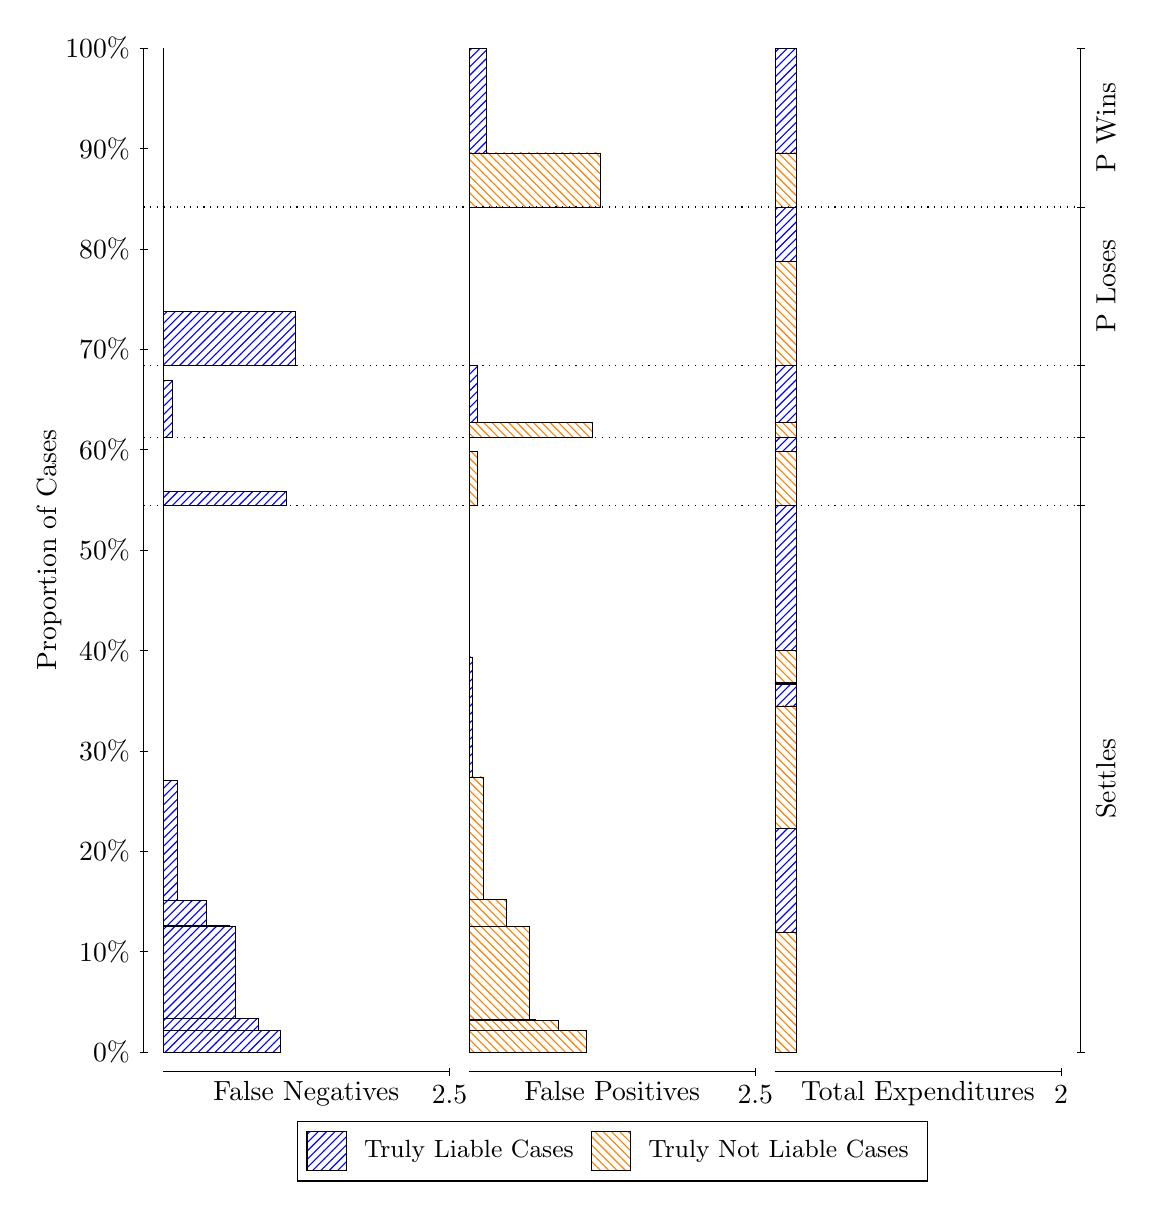
\begin{tikzpicture}
\draw[black, very thin] (1.5,1.75) -- (1.5,14.5);
\node[rotate=90, text=black, anchor=center] at (0.3, 8.125) {Proportion of Cases};
\draw[black, very thin] (1.45,1.75) -- (1.55,1.75);
\node[text=black, anchor=east] at (1.45, 1.75) {0\%};
\draw[black, very thin] (1.45,3.025) -- (1.55,3.025);
\node[text=black, anchor=east] at (1.45, 3.025) {10\%};
\draw[black, very thin] (1.45,4.3) -- (1.55,4.3);
\node[text=black, anchor=east] at (1.45, 4.3) {20\%};
\draw[black, very thin] (1.45,5.575) -- (1.55,5.575);
\node[text=black, anchor=east] at (1.45, 5.575) {30\%};
\draw[black, very thin] (1.45,6.85) -- (1.55,6.85);
\node[text=black, anchor=east] at (1.45, 6.85) {40\%};
\draw[black, very thin] (1.45,8.125) -- (1.55,8.125);
\node[text=black, anchor=east] at (1.45, 8.125) {50\%};
\draw[black, very thin] (1.45,9.4) -- (1.55,9.4);
\node[text=black, anchor=east] at (1.45, 9.4) {60\%};
\draw[black, very thin] (1.45,10.675) -- (1.55,10.675);
\node[text=black, anchor=east] at (1.45, 10.675) {70\%};
\draw[black, very thin] (1.45,11.95) -- (1.55,11.95);
\node[text=black, anchor=east] at (1.45, 11.95) {80\%};
\draw[black, very thin] (1.45,13.225) -- (1.55,13.225);
\node[text=black, anchor=east] at (1.45, 13.225) {90\%};
\draw[black, very thin] (1.45,14.5) -- (1.55,14.5);
\node[text=black, anchor=east] at (1.45, 14.5) {100\%};

\draw[black, very thin] (13.4,1.75) -- (13.4,14.5);
\draw[black, very thin] (13.35,1.75) -- (13.45,1.75);
\node[anchor=west] at (13.35, 1.75) {};
\draw[black, very thin] (13.35,8.6943) -- (13.45,8.6943);
\node[anchor=west] at (13.35, 8.6943) {};
\draw[black, very thin] (13.35,9.5526) -- (13.45,9.5526);
\node[anchor=west] at (13.35, 9.5526) {};
\draw[black, very thin] (13.35,10.471) -- (13.45,10.471);
\node[anchor=west] at (13.35, 10.471) {};
\draw[black, very thin] (13.35,12.481) -- (13.45,12.481);
\node[anchor=west] at (13.35, 12.481) {};
\draw[black, very thin] (13.35,14.5) -- (13.45,14.5);
\node[anchor=west] at (13.35, 14.5) {};

\draw[black, very thin, pattern color=blue, pattern=north east lines] (1.75,1.75) rectangle (3.2397,2.0281);
\draw[black, very thin, pattern color=blue, pattern=north east lines] (1.75,2.0281) rectangle (2.949,2.1747);
\draw[black, very thin, pattern color=blue, pattern=north east lines] (1.75,2.1747) rectangle (2.6583,3.3459);
\draw[black, very thin, pattern color=blue, pattern=north east lines] (1.75,3.3459) rectangle (2.5857,3.3564);
\draw[black, very thin, pattern color=blue, pattern=north east lines] (1.75,3.3564) rectangle (2.295,3.677);
\draw[black, very thin, pattern color=blue, pattern=north east lines] (1.75,3.677) rectangle (1.9317,5.2019);
\draw[black, very thin, pattern color=orange, pattern=north west lines] (1.75,5.2019) rectangle (1.75,8.6943);
\draw[black, very thin, pattern color=blue, pattern=north east lines] (1.75,8.6943) rectangle (3.3123,8.8711);
\draw[black, very thin, pattern color=orange, pattern=north west lines] (1.75,8.8711) rectangle (1.75,9.5526);
\draw[black, very thin, pattern color=blue, pattern=north east lines] (1.75,9.5526) rectangle (1.859,10.281);
\draw[black, very thin, pattern color=orange, pattern=north west lines] (1.75,10.281) rectangle (1.75,10.471);
\draw[black, very thin, pattern color=blue, pattern=north east lines] (1.75,10.471) rectangle (3.4213,11.157);
\draw[black, very thin, pattern color=orange, pattern=north west lines] (1.75,11.157) rectangle (1.75,12.481);
\draw[black, very thin, pattern color=orange, pattern=north west lines] (1.75,12.481) rectangle (1.75,13.168);
\draw[black, very thin, pattern color=blue, pattern=north east lines] (1.75,13.168) rectangle (1.75,14.5);
\draw[black, very thin, pattern color=orange, pattern=north west lines] (5.6333,1.75) rectangle (7.123,2.0209);
\draw[black, very thin, pattern color=orange, pattern=north west lines] (5.6333,2.0209) rectangle (6.7597,2.1549);
\draw[black, very thin, pattern color=orange, pattern=north west lines] (5.6333,2.1549) rectangle (6.469,2.1651);
\draw[black, very thin, pattern color=orange, pattern=north west lines] (5.6333,2.1651) rectangle (6.3963,3.3416);
\draw[black, very thin, pattern color=orange, pattern=north west lines] (5.6333,3.3416) rectangle (6.1057,3.6898);
\draw[black, very thin, pattern color=orange, pattern=north west lines] (5.6333,3.6898) rectangle (5.815,5.2425);
\draw[black, very thin, pattern color=blue, pattern=north east lines] (5.6333,5.2425) rectangle (5.6697,6.7674);
\draw[black, very thin, pattern color=blue, pattern=north east lines] (5.6333,6.7674) rectangle (5.6333,8.6943);
\draw[black, very thin, pattern color=orange, pattern=north west lines] (5.6333,8.6943) rectangle (5.7423,9.3758);
\draw[black, very thin, pattern color=blue, pattern=north east lines] (5.6333,9.3758) rectangle (5.6333,9.5526);
\draw[black, very thin, pattern color=orange, pattern=north west lines] (5.6333,9.5526) rectangle (7.1957,9.7424);
\draw[black, very thin, pattern color=blue, pattern=north east lines] (5.6333,9.7424) rectangle (5.7423,10.471);
\draw[black, very thin, pattern color=orange, pattern=north west lines] (5.6333,10.471) rectangle (5.6333,11.795);
\draw[black, very thin, pattern color=blue, pattern=north east lines] (5.6333,11.795) rectangle (5.6333,12.481);
\draw[black, very thin, pattern color=orange, pattern=north west lines] (5.6333,12.481) rectangle (7.3047,13.168);
\draw[black, very thin, pattern color=blue, pattern=north east lines] (5.6333,13.168) rectangle (5.8513,14.5);
\draw[black, very thin, pattern color=orange, pattern=north west lines] (9.5167,1.75) rectangle (9.7892,3.2747);
\draw[black, very thin, pattern color=blue, pattern=north east lines] (9.5167,3.2747) rectangle (9.7892,4.5926);
\draw[black, very thin, pattern color=orange, pattern=north west lines] (9.5167,4.5926) rectangle (9.7892,6.1452);
\draw[black, very thin, pattern color=blue, pattern=north east lines] (9.5167,6.1452) rectangle (9.7892,6.4233);
\draw[black, very thin, pattern color=orange, pattern=north west lines] (9.5167,6.4233) rectangle (9.7892,6.4335);
\draw[black, very thin, pattern color=blue, pattern=north east lines] (9.5167,6.4335) rectangle (9.7892,6.444);
\draw[black, very thin, pattern color=orange, pattern=north west lines] (9.5167,6.444) rectangle (9.7892,6.8489);
\draw[black, very thin, pattern color=blue, pattern=north east lines] (9.5167,6.8489) rectangle (9.7892,8.6943);
\draw[black, very thin, pattern color=orange, pattern=north west lines] (9.5167,8.6943) rectangle (9.7892,9.3758);
\draw[black, very thin, pattern color=blue, pattern=north east lines] (9.5167,9.3758) rectangle (9.7892,9.5526);
\draw[black, very thin, pattern color=orange, pattern=north west lines] (9.5167,9.5526) rectangle (9.7892,9.7424);
\draw[black, very thin, pattern color=blue, pattern=north east lines] (9.5167,9.7424) rectangle (9.7892,10.471);
\draw[black, very thin, pattern color=orange, pattern=north west lines] (9.5167,10.471) rectangle (9.7892,11.795);
\draw[black, very thin, pattern color=blue, pattern=north east lines] (9.5167,11.795) rectangle (9.7892,12.481);
\draw[black, very thin, pattern color=orange, pattern=north west lines] (9.5167,12.481) rectangle (9.7892,13.168);
\draw[black, very thin, pattern color=blue, pattern=north east lines] (9.5167,13.168) rectangle (9.7892,14.5);
\draw[black, dotted] (1.5,8.6943) -- (13.4,8.6943);
\draw[black, dotted] (1.5,9.5526) -- (13.4,9.5526);
\draw[black, dotted] (1.5,10.471) -- (13.4,10.471);
\draw[black, dotted] (1.5,12.481) -- (13.4,12.481);
\draw[black, very thin] (1.75,1.5) -- (5.3833,1.5);
\node[text=black, anchor=north] at (3.5667, 1.5) {False Negatives};
\draw[black, very thin] (5.3833,1.45) -- (5.3833,1.55);
\node[text=black, anchor=north] at (5.3833, 1.45) {2.5};

\draw[black, very thin] (5.6333,1.5) -- (9.2667,1.5);
\node[text=black, anchor=north] at (7.45, 1.5) {False Positives};
\draw[black, very thin] (9.2667,1.45) -- (9.2667,1.55);
\node[text=black, anchor=north] at (9.2667, 1.45) {2.5};

\draw[black, very thin] (9.5167,1.5) -- (13.15,1.5);
\node[text=black, anchor=north] at (11.333, 1.5) {Total Expenditures};
\draw[black, very thin] (13.15,1.45) -- (13.15,1.55);
\node[text=black, anchor=north] at (13.15, 1.45) {2};

\node[text=black, centered, rotate=90] at (13.72, 5.2222) {\contour{white}{Settles}};


\node[text=black, centered, rotate=90] at (13.72, 11.476) {\contour{white}{P Loses}};
\node[text=black, centered, rotate=90] at (13.72, 13.49) {\contour{white}{P Wins}};

\draw (7.449999999999999,1.5) node[draw=none] (baseCoordinate) {};
\begin{scope}[align=center]
        \matrix[scale=0.5, draw=black, below=0.5cm of baseCoordinate, nodes={draw}, column sep=0.1cm]{
            \node[rectangle, draw, minimum width=0.5cm, minimum height=0.5cm, pattern color=blue, pattern=north east lines] {}; &
            \node[draw=none, font=\small, text=black] (B) {Truly Liable Cases}; &
            \node[rectangle, draw, minimum width=0.5cm, minimum height=0.5cm, pattern color=orange, pattern=north west lines] {}; &
            \node[draw=none, font=\small, text=black] (B) {Truly Not Liable Cases}; \\
            };
\end{scope}

\end{tikzpicture}
\end{document}